                                                                                                        %\pdfoutput=1
%\documentclass[fms,times]{cuparticle}
\documentclass[a4paper,11pt,twoside]{amsart}
\usepackage{amsmath}
\usepackage{geometry}
%\newproof{proof}{Proof}
\usepackage{amssymb, latexsym}
\usepackage{appendix}
\usepackage{verbatim}
%\usepackage{amscd}
\usepackage{enumerate}
\usepackage{comment}
\usepackage{txfonts}
\usepackage{float}
\usepackage{parskip}
\usepackage{lipsum}
%\usepackage[breaklinks=true,hidelinks]{hyperref}

%\usepackage{psfig}
%\usepackage{graphicx}
%\usepackage{showkeys}  
%\usepackage{siunitx}
%\usepackage{tikz-cd}
%\usepackage{color}
%\usetikzlibrary{arrows}
% uncomment this when editing cross-references
%\numberwithin{equation}{section}
%\usepackage{hyperref}

%\volume{}
%\doi{}


% \usepackage{mathabx}


\usepackage{mathtools}%                  http://www.ctan.org/pkg/mathtools
\usepackage[tableposition=top]{caption}% http://www.ctan.org/pkg/caption
\usepackage{booktabs,dcolumn}%           http://www.ctan.org/pkg/dcolumn + http://www.ctan.org/pkg/booktabs
\usepackage[symbol]{footmisc}

\geometry{a4paper,total={6in,8in}, margin=1in}
\interfootnotelinepenalty=10000
     
%\theoremstyle{plain}

\newtheorem{theorem}{Theorem}[section]
%\newtheorem{theorem}[theorem]{Theorem}
\newtheorem{proposition}[theorem]{Proposition}
\newtheorem{hypothesis}[theorem]{Hypothesis}
\newtheorem{lemma}[theorem]{Lemma}
\newtheorem{corollary}[theorem]{Corollary}
\newtheorem{conjecture}[theorem]{Conjecture}
\newtheorem{principle}[theorem]{Principle}
\newtheorem{claim}[theorem]{Claim}

%\theoremstyle{definition}

%\newtheorem{roughdef}[subsection]{Rough Definition}
\newtheorem{definition}[theorem]{Definition}
\newtheorem{remark}[theorem]{Remark}
\newtheorem{remarks}[theorem]{Remarks}
\newtheorem{example}[theorem]{Example}
\newtheorem{examples}[theorem]{Examples}
%\newtheorem{problem}[subsection]{Problem}
%\newtheorem{question}[subsection]{Question}

\newcommand\F{\mathbb{F}}
\newcommand\E{\mathbb{E}}
\newcommand\R{\mathbb{R}}
\newcommand\Z{\mathbb{Z}}
\newcommand\N{\mathbb{N}}
\newcommand\D{\mathbb{D}}
\newcommand\C{\mathbb{C}}
\newcommand\Q{\mathbb{Q}}
\newcommand\T{\mathbb{T}}

\newcommand\e{\mathrm{e}}
\newcommand\Ei{\mathrm{Ei}}
\newcommand\IZi{\mathrm{IZi}}
\newcommand\li{\mathrm{li}}
\newcommand\Li{\mathrm{Li}}
\newcommand\Zi{\mathrm{Zi}}
\newcommand\PV{\mathrm{PV}}
\newcommand\Res{\mathrm{Res}}
\newcommand\RZi{\mathrm{RZi}}
\newcommand\sech{\mathrm{sech}}
\newcommand{\sgn}{\text{sgn}}

\renewcommand\Re{{\operatorname{Re\,}}}
\renewcommand\Im{{\operatorname{Im\,}}}
\renewcommand{\thefootnote}{\fnsymbol{footnote}}
\newcommand\Log{{\operatorname{Log}}}
\newcommand\eps{\varepsilon}



\renewcommand\P{\mathbf{P}}


%%%%%%%%%%%%%%%%%%%%%%%%%%%%%%%%


\newcommand{\alert}[1]{{\bf \color{red} TODO: #1}}


\setlength\evensidemargin\oddsidemargin
%\setlength{\parindent}{0cm}

\usepackage{color}
\definecolor{almond}{rgb}{0.94,0.87,0.8}

\let\oldv\verbatim
\let\oldendv\endverbatim

\def\verbatim{\par\setbox0\vbox\bgroup\oldv}
\def\endverbatim{\oldendv\egroup\fboxsep0pt \noindent\colorbox[gray]{0.8}{\usebox0}\par}

\begin{document}
\title[Roots of integrals of powers of the Riemann Zeta-function]{EXPLORING THE ROOTS OF THE INTEGRALS OF POWERS OF THE RIEMANN ZETA-FUNCTION}

\author{Dolph Dwars, Kalpesh Muchhal}
\date{\today, v1.2}
\address{\tt{{\it E-mail Address}: ra.dwars@quicknet.nl}}
\address{\tt{{\it E-mail Address}: kalpesh.muchhal@iitbombay.org}}

%%% AMS subject classification
\subjclass[2010]{Primary 33E20, 11Z05}
% 33-XX Special functions
% 33Exx      Other special functions
% 33E20  	 Other functions defined by series and integrals
%
% 11-XX Number theory
% 11Mxx	     Zeta and $L$-functions: analytic theory
%   11M06    $\zeta (s)$ and $L(s, \chi)$

\keywords{Riemann zeta function, Contour integration, Laurent series, Fractional calculus}

\begin{abstract}
The Riemann zeta-function $\zeta(s)$ shares the property with $\dfrac{1}{\log x}$ of having a simple pole at 1. In this paper we will apply the tools developed for the evaluation of $\displaystyle L(y,x) = \int_0^x \frac{1}{\log^{y} t}\, dt$ to $\displaystyle \Zi(y,x)=\int_0^x \zeta(t)^{y}\, dt$ for $x>1$. For $y < -0.5$ or $y > 0.5$, $\Zi(y,x)$ shows interesting properties which we explore both numerically and analytically. Some of the analysis will be repeated, but the main focus is on presenting and interpreting the results. Similar to the Ramanujan-Soldner constant, we present a possibly new zero for the case for $y=1$. We also present an expression for the evaluation of the multiple and fractional integrals (and derivatives) of $\zeta(s)$ for $y=1$. 
\end{abstract}

\maketitle

\section{Introduction}

In our recent paper \cite{mudw}, we developed tools to evaluate $L(n,x) = \int_0^x \frac{1}{\log^{y} t} dt$ for values of $x$ 'passing' the pole at $x=1$. These tools proved to be quite generic and therefore could be applied to other functions with a simple pole at $x=1$. Candidate functions are for instance $\frac{s}{s-1}$, and also the well known Riemann $\zeta(s)$ function \cite{edwr}. In this paper we will explore the integral and its roots for the latter, resulting in a few constants (similar to the Ramanujan-Soldner constant) that appear to be new.

There is abundant information available about the (log-)derivative(s) of $\zeta(s)$, however surprisingly little seems to be known about the integral of (powers) of $\zeta(s)$. Also, while $L(n,x)$ has a recursion relation, the same is not likely to exist for $\zeta(s)$. These differences and similarities have motivated us to start exploring:

\begin{equation}\label{zi1}
 \Zi(y,x) = PV \int_0^x {\zeta^{y}(t)} \,dt
\end{equation}


For a detailed analysis of the specific contour integration approach, we refer to our $\li$-paper \cite{mudw}, but in a nutshell; given an $y$ and $x$, we compute $\Zi(y,x)$ using several different contours to always arrive at the same estimate, showing that the Cauchy Principal Value, when computed this way, is a well defined concept even when higher order poles are involved. 
  
Some remarks on notation and convention used later in the paper:
\begin{itemize}
 \item exponent n $->$ emphasizes integer exponents
 \item exponent q $->$ emphasizes real exponents including integers
 \item PV, CPV $->$ Cauchy Principal Value obtained through complex integration 
 \item $\mu_y$ $->$ Solution of $\Zi(y,x)=0$
\end{itemize}

We will start our analysis for $y = n, x > 1$ using the Laurent series expansion of $\zeta(s)$ and then further develop it for $y = q$ and $x = z$. We also explore the fractional integral (and derivative) of $\zeta(s)$ for $y=1$.

\section{Laurent series expansion of $\zeta(s)$ for integer $n$}

Using the Laurent series expansion of $\zeta(z)$, we can use the multinomial theorem to obtain the corresponding expansion for $\zeta^{n}(s)$. This can then be used to easily get the residue for the latter expression at $z=1$.

Let $f(z)$ be a function with a simple pole, represented as a Laurent series as: $$f(z) = \frac{a_{-1}}{z-c} + a_0 + a_1 (z-c) + a_2 (z-c)^2 + ...$$
then $$(f(z))^n = \frac{1}{(z-c)^n} \sum\limits_{k=0}^{\infty}\left(\sum\limits_{\substack{t_{-1} + t_0 + t_1 + ... t_{k-1} = n \\ 0t_{-1} + 1t_0 + 2t_1 + ... kt_{k-1} = k}} \frac{n!}{t_{-1}!t_{0}!t_{1}!...t_{k-1}!} a_{-1}^{t_{-1}} a_{0}^{t_0}a_{1}^{t_1}..a_{k-1}^{t_{k-1}} (z-c)^k\right)$$

Extracting the coefficient of $(z-c)^{-1}$, we get:
$$\Res((f(z))^n,c) =  
\sum\limits_{\substack{t_{-1} + t_0 + t_1 + ... t_{n-2} = n \\ 0t_{-1} + 1t_0 + 2t_1 + ... (n-1)t_{n-2} = n-1}} \frac{n!}{t_{-1}!t_{0}!t_{1}!...t_{n-2}!} a_{-1}^{t_{-1}} a_{0}^{t_0}a_{1}^{t_1}..a_{n-2}^{t_{n-2}}$$
 
Also since,\\
$\zeta(z) = \frac{1}{z-1} + \sum\limits_{n=0}^{\infty} (-1)^n\,\frac{(z-1)^n}{n!}\, \gamma_n = \frac{1}{z-1} + \gamma_0 - \frac{\gamma_1}{1!}(s-1) + \frac{\gamma_2}{2!}(s-1)^2 - \frac{\gamma_3}{3!}(s-1)^3 \cdots$

we can tabulate the residues at $z=1$ for the first few power terms. Note that $\gamma_n$ are the Stieltjes constants. 

\begin{table}[H]
  \begin{center}
    \caption{Residues of a function's powers in terms of Laurent coefficients of the function}
    \label{tab:table1}
    \begin{tabular}{r|r|r|r} % <-- Alignments: 1st column left, 2nd middle and 3rd right, with vertical lines in between
      $n$ & $\Res((f(z))^n,c)$ &  $\Res(\zeta(z)^{n},1)$ & Numerical Value\\
      \hline
      1 &  $a_{-1}$ & 1 & 1.00000\\
      2 &  $2a_{-1}a_{0}$ & $2\gamma_0$ & 1.15443\\
      3 &  $3a_{-1}^2 a_{1} + 3a_{-1} a_{0}^2$ & $3\gamma_0^2-3\gamma_1$ & 1.21798\\
      4 &  $4a_{-1}^3 a_{2} + 12a_{-1}^2 a_{0} a_{1} + 4a_{-1} a_{0}^3$ & $4\gamma_0^3-12\gamma_0\gamma_1 +2\gamma_2$ & 1.25425\\
      .. & .. & .. & ..\\
    \end{tabular}
  \end{center}
\end{table}


\section{Roots of $\Zi(n,x)$ for integer $n$}

Since $\zeta(s)^{n}$ has a lone singularity at $1$, this allows us to numerically compute for any $x>1$, and could use any root finding method (eg. the bijection method) to search for roots of $\Zi(n,x)$.

\begin{figure}[H]
  \includegraphics[width=0.8\linewidth]{RootsZinx.png}
  \caption{Roots $\mu_n$ of $\Re(\Zi(n,x))$ for $n=1,2,3$ and $x > 1$}
\end{figure}

We find that $\Zi(1,x)$ has a single root $\mu_1 \approx 1.44726546099114$.., which appears to be a new constant that looks similar to the well known Ramanujan-Soldner's constant. We now calculate corresponding roots for $n>1$. As far as we know, these constants also appear to be new, and it remains to be seen whether they can be derived from other mathematical constants. 

Since for any $n \ge 1$, $\Zi(n,x)$ is monotonically increasing for $x>1$, $\Zi(n,x)$ always has a single root. Also as seen in the table below, the ratio of roots for consecutive $n$ seem to converge to $1$ when $n \rightarrow \infty$. 

\begin{table}[H]
  \begin{center}
    \caption{Roots of $\Zi(n,x)$}
    \label{tab:table2}
    \begin{tabular}{r|r|r|r|r} % <-- Alignments: 1st column left, 2nd middle and 3rd right, with vertical lines in between
      $n$ & $\mu_{n}$ & $\frac{\mu_{n}}{\mu_{n-1}}$\\
      \hline
      1 & 1.447265 & \\
      2 & 2.476428 & 1.711108\\
      3 & 2.989319 & 1.207108\\
      4 & 3.416343 & 1.142849\\
      5 & 3.728337 & 1.091324\\
      6 & 3.993442 & 1.071105\\
      .. & .. & ..\\
      300 & 9.650548652 & 1.000500\\
      301 & 9.655355581 & 1.000498\\
      .. & .. & ..\\
    \end{tabular}
  \end{center}
\end{table}

These roots $\mu_{n}$ can be used to derive a few interesting series expressions. For instance, for $x > 1$, we have for $n = 1$ the following integral expression:

\begin{equation}\label{zetPV1}
 PV \int_0^x \zeta(t)\, dt = PV \int_0^{\mu_1} \zeta(t)\, dt + \int_{\mu_1}^{x} \zeta(t)\, dt = \int_{\mu_1}^{x} \zeta(t) dt
\end{equation}

Since $\mu_1 > 1$ we can integrate the standard zeta-series $\displaystyle \sum_{n=1}^{\infty} \frac{1}{n^s}$ term by term and sum:

\begin{equation}\label{zetPV2}
  PV \int_0^x \zeta(t)\, dt = x - \mu_1 - \sum_{n=2}^{\infty} \frac{n^{-x}-n^{-\mu_1}}{\log(n)}
\end{equation}

The terms dependent on $x$ in the RHS, can be incorporated in a slightly altered integral on the LHS and we obtain:
\begin{equation}\label{zetPV3}
  PV \int_0^{\infty} (\zeta(t) - 1) \,dt = -\mu_1+\sum_{n=2}^{\infty} \frac{n^{-\mu_1}}{\log(n)}=-0.24323834...
\end{equation}

The above can be extended to higher powers, e.g, for $n=2$ we have the root $\mu_{2} = 2.476428..$:

\begin{equation}\label{zetPV4}
 PV \int_0^{\infty} (\zeta^{2}(t) - 1) \,dt = -\mu_{2} + \mathop{\sum_{k=1}^{\infty}\sum_{j=1}^{\infty}}_{kj \ne 1} \frac{(kj)^{-\mu_{2}}}{\log(kj)}\\
= -\mu_{2}+\sum_{k=2}^{\infty} \frac{k^{-2\,\mu_{2}}}{2\,\log(k)} + \mathop{\sum_{k=1}^{\infty}\sum_{j=1}^{\infty}}_{k \ne j} \frac{(kj)^{-\mu_{2}}}{\log(kj)} = -1.658841339... 
\end{equation}

In general, 
\begin{equation}\label{zetPV5}
 PV \int_0^{\infty} (\zeta^{n}(t) - 1) \,dt = -\mu_{n} + \mathop{\sum_{k_{1}=1}^{\infty}\sum_{k_{2}=1}^{\infty}..\sum_{k_{n}=1}^{\infty}}_{k_{1}k_{2}..k_{n} \ne 1} \frac{(k_{1}k_{2}..k_{n})^{-\mu_{n}}}{\log(k_{1}k_{2}..k_{n})}
\end{equation}

It also works for negative $y$, e.g. the integral of $\frac{1}{\zeta(x)}$ has zero $\mu_{-1} = 2.6179789..$ and its series expression is:

\begin{equation}\label{zetPV6}
 \int_0^x \frac{1}{\zeta(t)}\, dt = x- \mu_{-1} - \sum_{n=2}^{\infty} \mu(n)\frac{n^{-x}-n^{-\mu_{-1}}}{\log(n)}
\end{equation}

with $\mu(n)$ the Möbius function. We then obtain a similar equation as before:

\begin{equation}\label{zetPV7}
  \int_0^{\infty} \left(\frac{1}{\zeta(t)} -1\right) \,dt = -\mu_{-1}+\sum_{n=2}^{\infty} \mu(n)\frac{n^{-\mu_{-1}}}{\log(n)} = -2.9112576...
\end{equation}

While expressions involving the roots $\mu_n$ can be related to expressions involving the Stieltjes constants (through the Laurent expansion of $\zeta(s)$), such relations seem difficult to simplify. We have not found any closed form expressions for $\mu_n$ in terms of known mathematical constants.

\section{Laurent series expansion of $\zeta(s)^q$ for real $q$}
When $q$ is real but not necessarily an integer, the singularity at x=1 for $\zeta(s)$ is no longer a pole, but a branch point. Calculating the residue using the $(q-1)$th derivative approach is no longer feasible. But as demonstrated below, a function raised to a fractional or real exponent still has a Laurent series expansion, which can be used for residue extraction.

As in the previous section, let $f(z)$ have a simple pole (without loss of generality assumed to be at 0), and represented as a Laurent series as:
$$f(z) = \frac{a_{-1}}{z} + a_0 + a_1 z + a_2 z^2 + ...$$

and $q$ be a real number. Then:
\begin{align}
(f(z))^q &= (\frac{a_{-1}}{z} + a_0 + a_1 z + a_2 z^2 + ...)^q \notag\\
&= (a_0 + (\frac{a_{-1}}{z} + a_1 z + a_2 z^2 + ...))^q\notag\\
&= (a_0 + g(z))^q\notag\\
&= a_{0}^q + (q)_{1} a_{0}^{(q-1)} g(z) + \frac{(q)_{2}}{2!} a_{0}^{(q-2)} (g(z))^2 + \frac{(q)_{3}}{3!} a_{0}^{(q-3)} (g(z))^3 + ...\notag
\notag
\end{align}
where $(q)_k = q(q-1)(q-2)...(q-k+1)$.

This expansion has only integer exponents of $z$. Collecting the coefficients of $1/z$, we also see that $(g(z))^2$ does not contribute to the $1/z$ term.

Coefficient of $\frac{1}{z} = (q)_{1} a_{0}^{(q-1)} a_{-1} + \frac{(q)_{3}}{3!} a_{0}^{(q-3)} (3 a_{-1}^2 a_1) + \frac{(q)_{4}}{4!} a_{0}^{(q-4)} (4 a_{-1}^3 a_2) + \frac{(q)_{5}}{5!} a_{0}^{(q-5)} (5 a_{-1}^4 a_3 + 10 a_{-1}^3 a_{1}^2) + ...$

Generalizing to the pole at c, and making the expression more compact, we get: 
$$\Res((f(z))^q,c) = \sum\limits_{\substack{k=1 \\ k \ne 2}}^{\infty} \left(\frac{(q)_{k}}{k!} a_{0}^{(q-k)} \left(\sum\limits_{\substack{t_{-1} + t_1 + t_2 + ... t_{k-2} = k \\ -t_{-1} + 1t_0 + 2t_1 + ... (k-2)t_{k-2} = -1}} \frac{k!}{t_{-1}!t_{1}!...t_{k-2}!} a_{-1}^{t_{-1}} a_{1}^{t_1}..a_{k-2}^{t_{k-2}}\right)\right)$$

Since this is a general formula for real $q$, it is applicable for both integer and non integer exponents.

We first observe that for integer exponents, $(q)_k = 0$ for $k>q$, and we get the same closed form expression for the residue as in the earlier section.\\
For e.g. $q=4$, $\Res((f(z))^q,c) = 4 a_{0}^3 a_{-1} + \binom(4,3) a_0 (3 a_{-1}^2 a_1) + \binom(4,4) (4 a_{-1}^3 a_2)$
$=4 a_{0}^3 a_{-1} + 12 a_0 a_{-1}^2 a_1 + 4 a_{-1}^3 a_2)$

But for non-integer exponents, $(q)_k \ne 0$, and the residue formula is now an infinite series, thus the residue can be computed only approximately.

Also, we observe that if all the $a_i$ coefficients of the base function $f(z)$ are real, and $a_0 > 0$, then the residue for $f^{q}(z)$ also stays real. 

Additionally, since the inner sum formula is independent of $q$, only the $(q)_k a_{0}^{(q-k)}$ terms change on varying q. Since $\frac{(q+1)_k}{(q)_k} \to 1$ as q increases, if $0 < a_0 < 1$, the residue expression should have a tendency of faster convergence for higher $q$. 

Letting $f(z) = \frac{1}{z-1} + \sum\limits_{n=0}^{\infty} (-1)^n\,\frac{(z-1)^n}{n!}\, \gamma_n = \frac{1}{z-1} + \gamma_0 - \frac{\gamma_1}{1!}(s-1) + \frac{\gamma_2}{2!}(s-1)^2 + \frac{\gamma_3}{3!}(s-1)^3 \cdots$ we see that $a_0 = \gamma_0$, hence $\Res(\zeta(z)^{q},1)$ is real for $q$ real.

\begin{table}[H]
  \begin{center}
    \caption{Sample $\Res(\zeta(z)^{q},1)$ for real $q$}
    \label{tab:table3}
    \begin{tabular}{r|c|c|c} 
      $q$ & $\Res(\zeta(z)^{q},1)$ using formula & $\Res(\zeta(z)^{q},1)$ using numerical method & Remark\\
      \hline
      1.5 & 1.09844 & 1.13992\\
      2.0 & 1.15443 & 1.15443 & exact at integers\\
      2.5 & 1.19139 & 1.17874\\
      3.0 & 1.21798 & 1.21798 & exact at integers\\
      3.5 & 1.23822 & 1.24273\\
      ..
      4.5 & 1.26732 & 1.26557 \\
      ..
      10.5 & 1.33786 & 1.33784 \\ 
    \end{tabular}
  \end{center}
\end{table}

As expected for non-integer q powers, we see better agreement between formula and numerical evaluation as q is taken higher, while slow or possibly non-convergence at low q, which should be investigated further.

\section{Roots $\mu_q$ of $\Zi(q,x)$ for real $q$}

\begin{table}[H]
  \begin{center}
    \caption{Roots of $\Zi(y,x)$ for real $y$}
    \label{tab:table4}
    \begin{tabular}{r|c|c} 
      $q$ & $\mu_{q}$ & $\frac{\mu_{q}}{\mu_{q-1}}$\\
      \hline
      0.501 & 1.00000785 & \\
      0.51 & 1.00069468 & \\
      0.55 & 1.01283228 & \\
      0.6 & 1.04060213 & \\
      0.7 & 1.11934849 & \\
      0.8 & 1.21727056 & \\
      0.9 & 1.32794564 & \\
      1.0 & 1.44726546 & \\
      1.1 & 1.57160033 & \\
      1.2 & 1.69741796 & \\
      1.3 & 1.82135635 & \\
      1.4 & 1.94044812 & \\
      1.5 & 2.05235021 & \\
      2.0 & 2.47642872 & 1.2066306 \\
      2.5 & 2.74694715 & 1.1092373 \\
      3.0 & 2.98931929 & 1.0882332 \\
      3.5 & 3.22099071 & 1.0774997 \\
      4.0 & 3.41634327 & 1.0606498 \\
      4.5 & 3.57945275 & 1.0477438 \\
    \end{tabular}
  \end{center}
\end{table}

Note that in the table above, roots have been calculated numerically using contour integration, without resorting to the fractional residue formula of the previous section.  We observe that as $q \to 0.5$, $\mu_{q} \to 1$. Since $\zeta(s)$ has a singularity at $1$, and $\Zi(q,x)$ was defined for $x>1$, this implies no roots of $\Zi(q,x)$ for $0 < q <=0.5$.

\begin{figure}[H]
  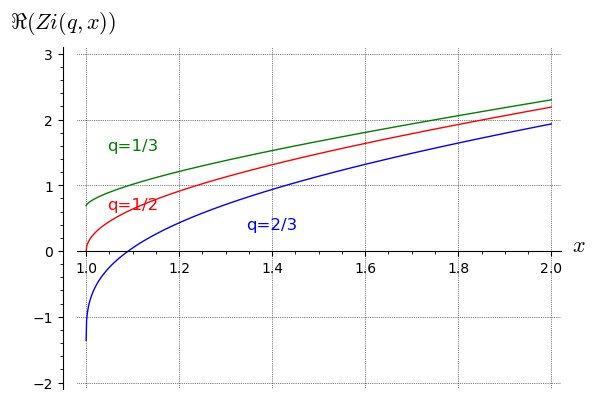
\includegraphics[width=0.8\linewidth]{RootsZiqx.png}
  \caption{Graphs of $\Re(\Zi(q,x)$ for $q=1/3,1/2,2/3$ and $x > 1$. There only exist $\mu_q$ for $q > 1/2$.}
\end{figure}

Additionally, it can be seen that the roots for fractional exponents interpolate well between those for integer exponents, and the ratio of roots with $q_{r} - q_{r-1} = 1$ still appears to converge towards $1$, further providing confirmation that the behaviour of $\Zi(q,x)$ is not fundamentally different between integer and non-integer exponents.

\section{$\Zi(y,z)$ for complex $z$}

In our analysis so far, we used the constraint $x > 1$. Given that $\zeta(s)$ can also be defined for $s$ complex, we now derive some expressions for the full analytic continuation $\Zi(y,z)$ defined everywhere except at $z=1$. We take three approaches based on globally convergent expressions for $\zeta(s)$.

The first approach uses the following integral \cite{zint}:
\begin{equation}\label{zetcom1}
  \zeta(s) = \frac{\pi}{s-1}\,\int_{-\infty}^{\infty} \left(\frac12+x\, i\right)^{1-s}\, \sech^2(\pi x) \, dx \qquad s \in \mathbb{C}, s \ne 1
\end{equation}

Next, take the integral of $\zeta(s)$ from $0...z$, however swap the order of integration as follows (assuming Fubini's theorem holds):
\begin{equation}\label{zetcom2}
  \Zi(1,z) = \int_0^z \zeta(s)\,ds =\pi \int_{-\infty}^{\infty} \sech^2(\pi x)\int_0^{z} \frac{\left(\frac12+x\, i\right)^{1-s} }{(s-1)} \, ds \, dx
\end{equation}

The inner $s$-integral can now be solved as follows:

\begin{equation}\label{zetcom3}
  \Zi(1,z) = -\frac{\pi}{2}\int_{-\infty}^{\infty} \sech^2(\pi x)\, \left( \Ei\left((1-z)\, \left(\frac{\pi i}{2}-\log\left(\frac{i}{2}+x\right) \right) \right) -\Ei\left(\frac{\pi i}{2}-\log \left(\frac{i}{2}+x\right) \right) \right) \, dx
\end{equation}

where $\Ei$ is the Exponential Integral \cite{expi}. The second $\Ei$ is independent of $z$, hence we could compute this integral once and replace it by the constant $0.2567616...$. We then obtain:
\begin{equation}\label{zetcom4}
  \Zi(1,z) = -\frac{\pi}{2}\int_{-\infty}^{\infty} \sech^2(\pi x)\, \Ei\left((1-z)\, \left(\frac{\pi i}{2}-\log\left(\frac{i}{2}+x\right) \right) \right)\, dx + 0.25676165710901...
\end{equation}

and this is valid for $z \in \mathbb{C}, z \ne 1, \Im(z) \ge 0$. We did not find a way to extend this towards $y \ne 1$.

Our second approach uses the well known Hasse/Ser series expression \cite{hase} for $\zeta(s)$:
\begin{equation}\label{zetcom5}
  \zeta(s) = \frac{1}{s-1} \sum_{n=1}^{\infty} \frac{1}{n} \sum_{k=1}^n \binom{n-1}{k-1}\,\frac{(-1)^{k-1}}{(k)^{s-1}} \qquad s \in \mathbb{C}, s \ne 1
\end{equation}

where after integration over $s$ we obtain:
\begin{equation}\label{zetcom6}
  \Zi(1,z) =\sum_{n=1}^{\infty} \frac{1}{n} \left(\sum_{k=2}^n(-1)^k\, \binom{n-1}{k-1}\,\left(\Ei\left(1,(z-1)\log(k)\right)-\Ei\left(1,-\log(k)\right)  \right)-\log\left(\frac{1}{1-z}\right)\right)
\end{equation}

Since the Logarithmic Integral $\Li(k) = -\Ei\left(1,-\log(k)\right)$ \cite{logi} and including $\pi i$ to accommodate the branch cut, we could also rewrite this as:
\begin{equation}\label{zetcom7}
  \Zi(1,z) = \sum_{n=1}^{\infty} \frac{1}{n}\left( \sum_{k=2}^n(-1)^k\, \binom{n-1}{k-1}\,\left(\Ei\left(1,(z-1)\log(k)\right)+\Li(k)\right) +\pi\,i -\log\left(\frac{1}{1-z}\right) \right) -\pi\,i
\end{equation}

Again, both are valid for $z \in \mathbb{C}, z \ne 0, \Im(z) \ge 0$. We did not yet find a way to extend this towards $y \ne 1$.

The third approach uses the Laurent series expansion for $\zeta(s)$ at $s=1$:
\begin{equation}\label{zetcom8}
  \zeta(s) = \frac{1}{s-1}+\sum_{n=0}^{\infty} \frac{\gamma_n}{n!}\,(1-s)^n \qquad s \in \mathbb{C}, s \ne 1
\end{equation}

where $\gamma_n$ are the Stieltjes constants \cite{stie}. Integration over $s$ for $y = n$, yields the following series expressions for indefinite integrals:

\begin{align}
\int \zeta(s)^{1} ds &= \log(s-1)\- - \sum_{n=1}^{\infty} \frac{1}{n}\cdot \binom{1}{1}\,\frac{\gamma_{n-1}}{(n-1)!}\,(1-s)^n \notag \\
\int \zeta(s)^{2} ds &= -\frac{1}{1\,(1-s)^1}+\log(t-1)\,2\gamma_0 + \sum_{n=1}^{\infty} \frac{1}{n}\cdot \left(\, \binom{2}{1}\,\frac{\gamma_{n}}{n!} -\binom{2}{2}\,\sum_{k=0}^{n-1} \frac{\gamma_k\,\gamma_{n-k-1}}{k!\,(n-k-1)!} \right)\,(1-s)^n \notag \\
\int \zeta(s)^{3} ds &= -\frac{1}{2\,(1-s)^2} - \frac{3\,\gamma_0}{s-1}- \log(t-1)\,\left(3\gamma_0^2+3\,\gamma_1\right) + \sum_{n=1}^{\infty} \frac{1}{n}\cdot \left(\, \binom{3}{1}\,\frac{\gamma_{n+1}}{(n+1)!} -\binom{3}{2}\,\sum_{k=0}^{n} \frac{\gamma_k\,\gamma_{n-k}}{k!\,(n-k)!} \right. \notag \\
& \quad \left. +\, \binom{3}{3}\,\sum_{l=0}^{n-1} \sum_{m=0}^{n-l-1} \frac{\gamma_l\,\gamma_m\,\gamma_{n-m-l-1}}{l!\,m!\,(n-m-l-1)!}  \right)\,(1-s)^n \notag \\
\cdots \notag 
\end{align}
These integrals could be made definite from limits $0$ to $z$ by simply subtracting $F(z) - F(0)$. These expansions are also valid for $z \in \mathbb{C}, z \ne 1, \Im(z) \ge 0$. So far, they only work for $y \in \mathbb{N}$ and higher $y$ become increasingly complicated to compute.

\begin{figure}[H]
  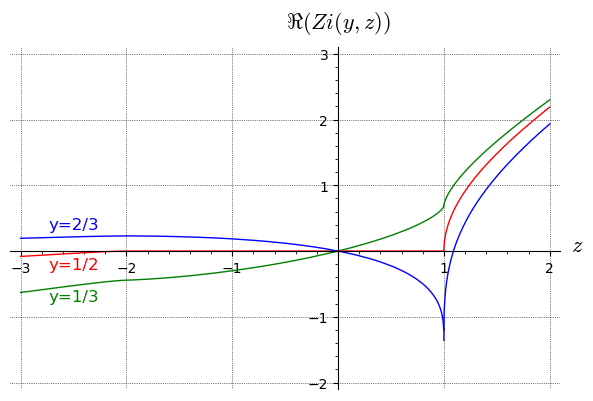
\includegraphics[width=0.9\linewidth]{AncontZizx.png}
  \caption{Continuation of $\Zi(y,z)$ for $z < 1$ with $y=1/3, 1/2, 2/3$. Observe that for $y = 1/2$, the function becomes purely imaginary in the range $-2 \le z < 1$. Values for $z < 1$ were computed through direct evaluation of the integral of the y-powers of $\zeta(s)$.}
\end{figure}

All three approaches could be used for numerical computations. Focusing only on the real part and making $y$ an integer: $\RZi(n,z) = \Re(\Zi(n,z))$ we see that $\RZi(n,z)$ has one zero on the positive axis for each $n$ (ref the earlier table) and an infinite number of zeros on the negative axis, however only when $n =$ odd. 

\begin{table}[H]
  \begin{center}
    \begin{tabular}{c|c|c|c} % <-- Alignments: 1st column left, 2nd middle and 3rd right, with vertical lines in between
      root of $\RZi(1,z)$ &root of $\RZi(2,z)$ & root of $\RZi(3,z)$ & root of $\RZi(4,z)$\\
      \hline
      (...) & none & (...) & none\\
      -26.52860 &&-26.31740\\
      -24.54619 &&-24.33145\\
      -22.56639 &&-22.34808\\
      -20.58734 &&-20.36814\\
      -18.63371 &&-18.39296\\
      -16.47823 &&-16.40254\\
      -15.28576 &&-15.03748\\
    \end{tabular}
  \end{center}
  \caption{Negative axis zeros of $\RZi(n,z)$. Subsequent zeros at increasingly negative $z$ appear to converge to some constant factor that is difficult to compute accurately.}
\end{table}
\vspace{-2em}

We also observe that the function $M(n,z) = \Zi(n,z) + \Zi(n,1-z)$ has an infinite number of complex roots, that we conjecture to all reside on the critical line $\Re(z)=0.5$ (at least within the critical strip, there could be a finite few outside the strip). The first zeros are listed below:

\begin{table}[H]
  \begin{center}
    \begin{tabular}{c|c|} % <-- Alignments: 1st column left, 2nd middle and 3rd right, with vertical lines in between
      root of $M(1,z)$ &root of $M(2,z)$\\
      \hline
		0.5000000000 + 0.601175154i & 0.5000000000 + 0.335971324i\\
		0.5000000000 + 7.449444039i & 0.5000000000 + 1.961276460i\\
		0.5000000000 + 11.43499027i & 0.5000000000 + 4.882815016i\\
		0.5000000000 + 16.19092846i & 0.5000000000 + 12.36083416i\\
		0.5000000000 + 19.45158106i & 0.5000000000 + 15.84975441i\\
		0.5000000000 + 26.23432187i & 0.5000000000 + 19.85884536i\\
		0.5000000000 + 34.24158919i & 0.5000000000 + 24.58528344i\\
		0.5000000000 + 39.11839760i & 0.5000000000 + 25.77196627i\\
		0.5000000000 + 46.84712903i & 0.5000000000 + 29.16409896i\\
		(...) &(...)\\
    \end{tabular}
  \end{center}
  \caption{Roots of $M(n,z)$. No clear pattern seems to be emerging.}
\end{table}
\vspace{-2em}


\section{Fractional integrals (and derivatives) of $\zeta(s)$}
  
Although we didn't find easy-to-compute expressions for the integral with powers $y \ne 1$ in $\zeta(s)^y$, it did prove worthwhile to explore double, triple,.. and fractional integrals for $y=1$. Starting from the R-L interpretation \cite{rili} of the fractional integral ($\alpha < 0$) of $\zeta(s)$, we found that the following equation:
\begin{equation}\label{zetfrac1}
 \zeta^{(\alpha)}(z) = \frac{1}{\Gamma(-\alpha)}\left(\frac{z^{-a}\,{}_{2}F_{1}\left(\left[1,-\alpha\right],\left[1-\alpha\right],\frac{z}{z-1}\right)}{\alpha\,(1-z)}-\frac{z^{-\alpha}}{2\,\alpha} +2^{-\alpha}\int_{0^+}^\infty \frac{(x^2+1)^{-z/2}}{\exp(2\,\pi\,x)-1}\,\left(k1(z,x,-\alpha)+k2(z,x,-\alpha)\right) \, dx\right)
\end{equation}

yields all fractional integrals over $0..z$ when $\alpha < 0$ and all fractional $z$-derivatives for $\alpha > 0, \alpha \in \mathbb{C}, z \in \mathbb{R}, z \ne 1$, except when $\alpha=0$ or a positive integer. It also works for $-\alpha \in \mathbb{N}/0, z \in \mathbb{C}, z \ne 1$. We have:
\begin{align}
f1(z,x) &= -i\,(1-x\,i)^{-z/2}\,(1+x\,i)^{z/2}, \quad f2(z,x) = i\,(1-x\,i)^{z/2}\,(1+x\,i)^{-z/2}\\
g1(x) &= 2\,\log(1-x\,i), \quad g2(x) = 2\,\log(1+x\,i)\\
k1(z,x,\alpha) &= f1(z,x)\,\left(\frac{\exp(-\sgn(\Re(z))\,\alpha\,\pi\,i))\,\Gamma(\alpha)}{g1(x)^{\alpha}} -(z/2)^{\alpha}\,\Ei(1-\alpha, -z/2\,g1(x)) \right)\\
k2(z,x,\alpha) &= f2(z,x)\,\left(\frac{\exp(\alpha\,\pi\,i))\,\Gamma(\alpha)}{g2(x)^{\alpha}} -(z/2)^{\alpha}\,\Ei(1-\alpha, -z/2\,g2(x)) \right)
\notag
\end{align}

This equation has been derived from the following integral for $\zeta(s)$ \cite{zeti}:

\begin{equation}\label{zetfrac2}
  \zeta(s) = \frac{1}{s-1}+\frac12+2\,\int_0^{\infty} \frac{\sin(s\,\arctan(x))}{(x^2+1)^{s/2}\,(\exp(2\,\pi\,x)-1)} \,dx \qquad s \in \mathbb{C}, s \ne 1
\end{equation}

Applying the Riemann-Liouville fractional integral gives:

\begin{equation}\label{zetfrac3}
  {}_0 I_z^{(\alpha)} \zeta(s) =\frac{1}{\Gamma(-\alpha)} \left( \int_0^z (z-s)^{-\alpha-1} \left( \frac{1}{s-1}+\frac12+2\,\int_0^{\infty} \frac{\sin(s\,\arctan(x))}{(x^2+1)^{s/2}\,(\exp(2\,\pi\,x)-1)} \,dx \right) \, ds \right)
\end{equation}

The integration of the $\frac{1}{s-1}$ and $\frac12$ terms is straightforward. In the third term the integrals could be swapped as follows (assuming Fubini's theorem applies):

\begin{equation}\label{zetfrac4}
 2\,\int_0^{\infty} \frac{1}{(\exp(2\,\pi\,x)-1)} \int_0^z \frac{\sin(s\,\arctan(x))}{(x^2+1)^{s/2}}\,(z-s)^{-\alpha-1} \,ds \, dx
\end{equation}


Mathematica\texttrademark{} evaluates the inner indefinite integral into closed form components, that can be evaluated for $z$ and $0$ resulting in the equation above. This expression allows for fast computations and we have computed the real roots of ${}_0 I_z^{(\alpha)} \zeta(s)$ for $z > 1$ up till the 11-th integral of $\zeta(s)$.:

\begin{table}[H]
  \begin{center}
    \caption{Roots of $\Re({}_0 I_z^{(\alpha)} \zeta(s))$}
    \label{tab:table5}
    \begin{tabular}{c|c|c} 
      $\alpha$ & Root of $\Re({}_0 I_z^{(\alpha)} \zeta(s))$ & $\Re({}_0 I_z^{(n)})-\Re({}_0 I_z^{(n-1)})$\\
      \hline
      -0.50 & 1.00000000000 & \\
      -0.75 & 1.18328684035 & \\
      -1.00 & 1.44726546099 & \\
      -1.25 & 1.72398154920 & \\
      -1.50 & 2.00433122969 & \\
      -1.75 & 2.28594756351 & \\
      -2.00 & 2.56803877198 & 1.1207733110 \\
      -2.25 & 2.85030136874 & \\
      -2.50 & 3.13261005146 & \\
      -2.75 & 3.41491170464 & \\
      -3.00 & 3.69718451134 & 1.1291457394 \\
      -4.00 & 4.82591052789 & 1.1287260166 \\
      -5.00 & 5.95415436080 & 1.1282438329 \\
      -6.00 & 7.08208537033 & 1.1279310095\\
      -7.00 & 8.20981556431 & 1.1277301940\\
      -8.00 & 9.33741202098 & 1.1275964567\\
      -9.00 &10.46491579697 & 1.1275037760\\
     -10.00 &11.59235302295 & 1.1274372260\\
     -11.00 &12.71974098629 & 1.1273879633\\
    \end{tabular}
  \end{center}
\end{table}
The difference between the real roots of subsequent integer values of $\alpha$ appears to converge to $1.127...$. It will require more work to establish a more precise value.
\begin{figure}[H]
  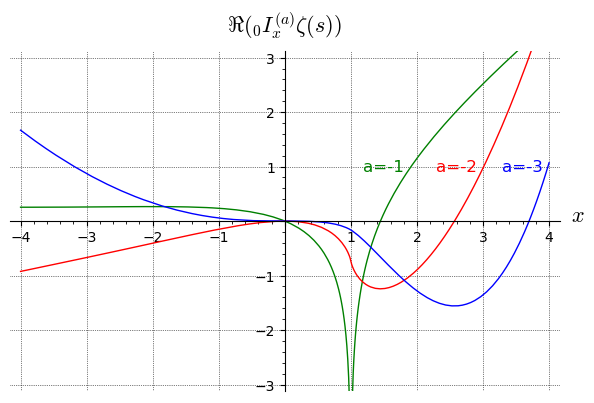
\includegraphics[width=0.9\linewidth]{fracintzeta.png}
  \caption{Real part roots of single $(\alpha=-1)$, double $(\alpha=-2)$ and triple $(\alpha=-3)$ integrals of $\zeta(s)$ over $0..x$. Note that the pole at $x=1$ vanishes for $\alpha < -1$ and induces new constants at that point. `For $\alpha=-2$ we get $-0.736789911..$, for $\alpha=-3$ we find $-0.1633480526...$}
\end{figure}


\begin{figure}[H]
  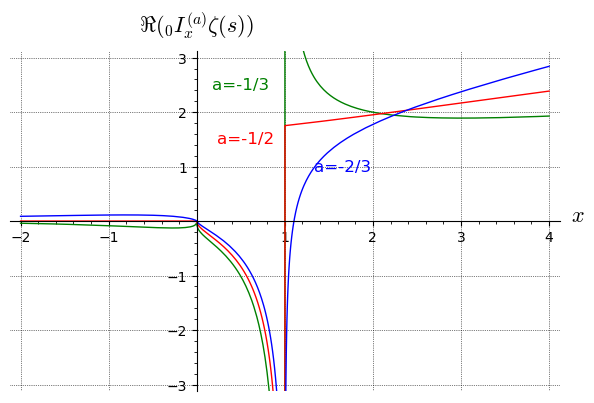
\includegraphics[width=0.9\linewidth]{fracintzeta1.png}
  \caption{Fractional integrals of $\zeta(s)$ for $\alpha=-1/3, -1/2, -2/3$. Note that the zeros in the region $x > 1$ only occur when $\alpha < -1/2$. Surprisingly a limiting real part value for $\alpha=-1/2$ at $x=1$ could be computed and it converges towards $1.751283864140..$}
\end{figure}


\begin{figure}[H]
  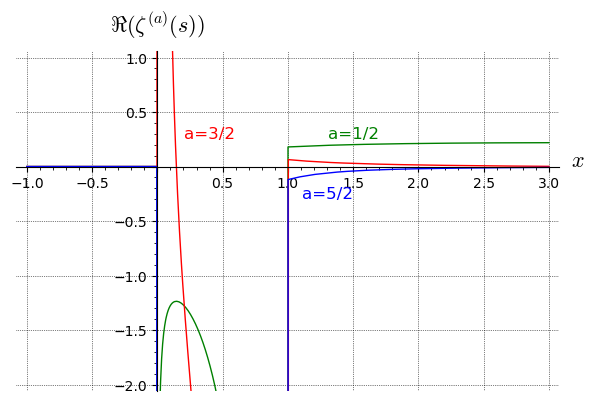
\includegraphics[width=0.9\linewidth]{fracderzeta.png}
  \caption{Fractional derivatives of $\zeta(x)$ for $\alpha=1/2, 3/2, 5/2$. We observe that for all $\alpha = n + 1/2$ the function becomes purely complex for all $ x < 0$}
\end{figure}

  
\section{Concluding Remarks and Future Work}

The analysis of the various integrals of $\zeta(s)^y$ demonstrates that they are fundamentally different from the integrals of $\frac{1}{\log x}^y$. The latter yielded expressions with finite series or even closed forms that were easy to expand to $y \ne 1$. For $\zeta(s)^{y}$, finding expressions for $y \ne 1$ and $x < 1$ proved to be tough, although direct evaluation of the integral in that domain (there is no longer a pole to avoid), obviously is a viable alternative for computations. We plan to further exploit the roots of the expression for the Riemann-Liouville fractional integrals/derivatives.

\begin{thebibliography}{99} 
\bibitem{mudw}
Muchhal K. and Dwars, R.A. \emph{Extending the logarithmic integral: An exploration of integrals of powers of the reciprocal of the log-function}, 2023
\bibitem{edwr}
Edwards, H.M. \emph{Riemann's zeta function}, 1974
\bibitem{rama}
Ramanujan, S, \emph{Collected Papers of Srinivasa Ramanujan}, Ed. G.H Hardy, P.V.S. Aiyar, B.M. Wilson. Providence, RI, Amer. Math. Soc., 2000, pg.351.
\bibitem{zint}
Milgram, Michael S.  \emph{Integral and Series Representations of Riemann's Zeta Function and Dirichlet's Eta Function and a Medley of Related Results}, Hindawi Journal of mathematics, 2013, p3 equation (14), which can be found at https://www.hindawi.com/journals/jmath/2013/181724/
\bibitem{hase}
Hasse, H, \emph{Ein Summierungsverfahren für die Riemannsche $\zeta$-Reihe}, Math. Z., 32 (1930), p 458–464.
\bibitem{expi}
Weisstein, Eric. W, \emph{Exponential Integral Ei}, From Mathworld A Wolfram Web Resource which can be found at: https://mathworld.wolfram.com/ExponentialIntegral.html
\bibitem{logi}
Weisstein, Eric. W, \emph{Logarithmic Integral}, From Mathworld A Wolfram Web Resource which can be found at: https://mathworld.wolfram.com/LogarithmicIntegral.html
\bibitem{stie}
Weisstein, Eric. W, \emph{Stieltjes Constants}, From Mathworld A Wolfram Web Resource which can be found at:   https://mathworld.wolfram.com/StieltjesConstants.html
\bibitem{rili}
Wikipedia, \emph{Riemann Liouville integral}, From Wikipedia, a Web Resource which can be found at:  https://
en.wikipedia.org/wiki/Riemann–Liouvilleintegral
\bibitem{zeti}
Digital Library of Mathematical Functions \emph{Integral representation of $\zeta(s)$}, From DLMF, 25.5.11	DLMF Web equation  Resource which can be found at:  https://dlmf.nist.gov/25.5
\end{thebibliography} 

\appendix
\appendixpage
The below codes are in parigp language. As a cautionary practice while copy-pasting code, do check whether special characters like \textasciicircum \, (power symbol) have been copied correctly. Note that several of the functions used here directly or as helpers such as intarc, fastresidue, getlaurent, ldsolve, tvectors and others were defined in the appendix of the li-paper.

\section{Numerically computing $\Zi(q,x)$ and $\Res(\zeta(z)^{q}, 1)$ for real $q$}
\begin{verbatim}
f(z,y) = zeta(z)^y;
g(x,y) = intnum(s=x,2,f(s,y));
cpvsemi(f,y) = Pi*I*intarc(1,1,0,Pi,f,y);
Zires(y) = imag(cpvsemi(f,y))/Pi;
Zi(y,x) = -real(cpvsemi(f,y) + g(x,y));

Example Computation
q=3.5;
x=4;
Zires(q)
Zi(q,x)

\end{verbatim}

\section{Calculating $\Res(\zeta^{q}(z), 1)$ for real q using laurent expansion formula}
Formula based results are calculated using the 'fastresidue' function. Compare 'fastresidue' results v/s 'Zires' results.\
They should be the same when q is an integer, different when q is non-integer, and align better as q increases.

\begin{verbatim}
laur30 = getlaurent(zeta,1,30);
[Zires(1.5), fastresidue(laur30,1.5)]
[Zires(3), fastresidue(laur30,3)]
[Zires(10.5), fastresidue(laur30,10.5)]
\end{verbatim}


\section{Calculating roots of $\Zi(n,x)$ for integer $n$}
With some easy modifications, the same can be done for real q as well, which we leave as an exercise for the reader.

\begin{verbatim}
{
zprev=1;
for(y=1,40,
   zero=solve(x=1.1,10^50,Zi(y,x));
   print(y,",",zero,",",zero/zprev);
   zprev=zero;
   );
}   
\end{verbatim}


\section{Evaluating the fractional integrals ($a <0$) and derivatives ($a > 0$) for $\zeta(s)$}

\begin{verbatim}
expint(p,z)= z^(p-1)*exp(-z)*hyperu(p,p,z); \\exponential integral E(p,z)

f1(z,x) = -I*(1-I*x)^(-z/2)*(1+I*x)^(z/2);
f2(z,x) = I*(1-I*x)^(z/2)*(1+I*x)^(-z/2);
g1(x)   = 2*log(1-I*x);
g2(x)   = 2*log(1+I*x);
m1(z,x,a) = (z/2)^a*expint(1-a,-z*g1(x)/2);
m2(z,x,a) = (z/2)^a*expint(1-a,-z*g2(x)/2);
t1(z,x,a) = exp(-sign(real(z))*a*Pi*I)*gamma(a)/(g1(x)^a)-m1(z,x,a);
t2(z,x,a) = exp(a*Pi*I)*gamma(a)/(g2(x)^a)-m2(z,x,a);
kt(z,x,a) = f1(z,x)*t1(z,x,-a) + f2(z,x)*t2(z,x,=a);

nin(z,a) = intnum(x=10^(-19),12,(x^2+1)^(-z/2)/(exp(2*Pi*x)-1)*kt(z,x,a));

pr(z,a)  = z^a*(hypergeom([1,a],[a+1],z/(z-1))/(a*(z-1))+ 1/(2*a));

zid(z,a) = if(a==0, zeta(z), 1/gamma(-a)*(pr(z,-a) + 2^(-a)*nin(z,-a)));
\end{verbatim}


\end{document}
